\documentclass[11pt,a4paper]{article}

            \usepackage[utf8]{inputenc}
            \usepackage[T1]{fontenc}
            \usepackage{lmodern}
            \usepackage[a4paper,margin=1.6cm]{geometry}
            \usepackage{graphicx}
            \usepackage{tikz}
            \usetikzlibrary{arrows.meta,positioning,fit,calc}
            \usepackage{tabularx}
            \usepackage{booktabs}
            \usepackage{array}
            \usepackage{enumitem}
            \usepackage{hyperref}
            \usepackage{xcolor}
            \usepackage{titlesec}
            \usepackage{ragged2e}
            \usepackage{setspace}
            \usepackage{float}

            \definecolor{navy}{HTML}{0B3954}
            \definecolor{teal}{HTML}{087E8B}
            \definecolor{gold}{HTML}{F4B942}
            \definecolor{coral}{HTML}{FF6B35}
            \definecolor{slate}{HTML}{34495E}
            \definecolor{softblue}{HTML}{EEF6FA}
            \definecolor{softteal}{HTML}{EAF7F8}
            \definecolor{softgold}{HTML}{FFF7E3}
            \definecolor{softgray}{HTML}{F7FAFC}

            \hypersetup{
              colorlinks=true,
              urlcolor=teal,
              linkcolor=navy,
              pdftitle={Model Dataflow Architecture},
              pdfauthor={Codex},
              pdfsubject={Data extraction and module mapping for market regime detection and RL allocation}
            }

            \setlength{\parindent}{0pt}
            \setlength{\parskip}{0.45em}
            \renewcommand{\arraystretch}{1.18}
            \onehalfspacing

            \titleformat{\section}{\Large\bfseries\color{navy}}{\thesection}{0.6em}{}
            \titleformat{\subsection}{\large\bfseries\color{teal}}{\thesubsection}{0.6em}{}

            \newcolumntype{Y}{>{\RaggedRight\arraybackslash}X}

            \begin{document}

            {\LARGE\bfseries\color{navy}Model Dataflow Architecture\par}
            {\large Repo-aligned extraction, feature engineering, and module mapping for market regime detection plus RL allocation\par}

            \section{End-to-End Diagram}

            \begin{figure}[H]
            \centering
            \scalebox{0.82}{
            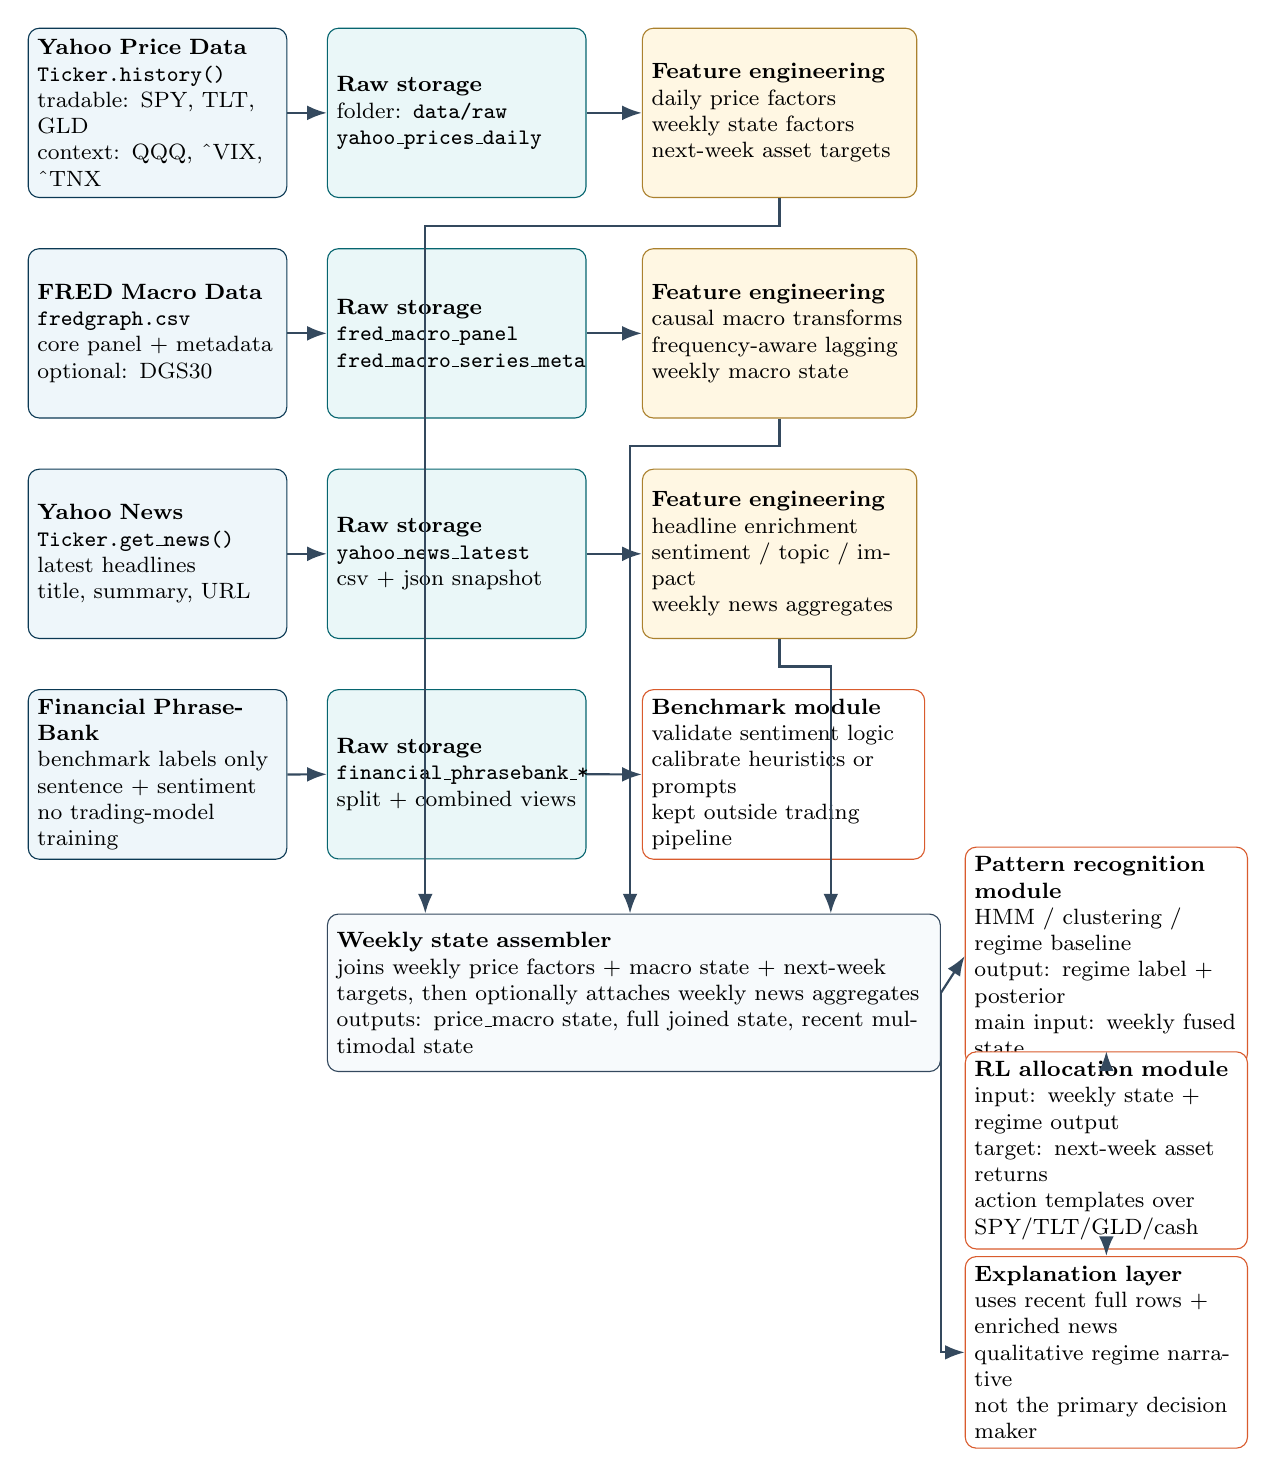
\begin{tikzpicture}[
              font=\footnotesize,
              x=1cm,
              y=1cm,
              >={Latex[length=2.5mm]},
              source/.style={draw=navy, fill=softblue, rounded corners, text width=3.05cm, minimum height=2.15cm, align=left, anchor=north west},
              raw/.style={draw=teal!80!black, fill=softteal, rounded corners, text width=3.05cm, minimum height=2.15cm, align=left, anchor=north west},
              feat/.style={draw=gold!70!black, fill=softgold, rounded corners, text width=3.25cm, minimum height=2.15cm, align=left, anchor=north west},
              module/.style={draw=coral!85!black, fill=white, rounded corners, text width=3.35cm, minimum height=2.15cm, align=left, anchor=north west},
              joinbox/.style={draw=slate, fill=softgray, rounded corners, text width=7.55cm, minimum height=2.0cm, align=left, anchor=north west},
              arrow/.style={->, thick, color=slate}
            ]
            \node[source] (price) at (0,0) {
              \textbf{Yahoo Price Data}\\
              \texttt{Ticker.history()}\\
              tradable: SPY, TLT, GLD\\
              context: QQQ, \textasciicircum{}VIX, \textasciicircum{}TNX
            };
            \node[source] (macro) at (0,-2.8) {
              \textbf{FRED Macro Data}\\
              \texttt{fredgraph.csv}\\
              core panel + metadata\\
              optional: DGS30
            };
            \node[source] (news) at (0,-5.6) {
              \textbf{Yahoo News}\\
              \texttt{Ticker.get\_news()}\\
              latest headlines\\
              title, summary, URL
            };
            \node[source] (phrasebank) at (0,-8.4) {
              \textbf{Financial PhraseBank}\\
              benchmark labels only\\
              sentence + sentiment\\
              no trading-model training
            };

            \node[raw] (rawprice) at (3.8,0) {
              \textbf{Raw storage}\\
              folder: \texttt{data/raw}\\
              \texttt{yahoo\_prices\_daily}
            };
            \node[raw] (rawmacro) at (3.8,-2.8) {
              \textbf{Raw storage}\\
              \texttt{fred\_macro\_panel}\\
              \texttt{fred\_macro\_series\_meta}
            };
            \node[raw] (rawnews) at (3.8,-5.6) {
              \textbf{Raw storage}\\
              \texttt{yahoo\_news\_latest}\\
              csv + json snapshot
            };
            \node[raw] (rawphrase) at (3.8,-8.4) {
              \textbf{Raw storage}\\
              \texttt{financial\_phrasebank\_*}\\
              split + combined views
            };

            \node[feat] (featprice) at (7.8,0) {
              \textbf{Feature engineering}\\
              daily price factors\\
              weekly state factors\\
              next-week asset targets
            };
            \node[feat] (featmacro) at (7.8,-2.8) {
              \textbf{Feature engineering}\\
              causal macro transforms\\
              frequency-aware lagging\\
              weekly macro state
            };
            \node[feat] (featnews) at (7.8,-5.6) {
              \textbf{Feature engineering}\\
              headline enrichment\\
              sentiment / topic / impact\\
              weekly news aggregates
            };
            \node[module] (modphrase) at (7.8,-8.4) {
              \textbf{Benchmark module}\\
              validate sentiment logic\\
              calibrate heuristics or prompts\\
              kept outside trading pipeline
            };

            \node[joinbox] (join) at (3.8,-11.25) {
              \textbf{Weekly state assembler}\\
              joins weekly price factors + macro state + next-week targets, then optionally attaches weekly news aggregates\\
              outputs: price\_macro state, full joined state, recent multimodal state
            };
            \node[module] (regime) at (11.9,-10.4) {
              \textbf{Pattern recognition module}\\
              HMM / clustering / regime baseline\\
              output: regime label + posterior\\
              main input: weekly fused state
            };
            \node[module] (rl) at (11.9,-13.0) {
              \textbf{RL allocation module}\\
              input: weekly state + regime output\\
              target: next-week asset returns\\
              action templates over SPY/TLT/GLD/cash
            };
            \node[module] (explain) at (11.9,-15.6) {
              \textbf{Explanation layer}\\
              uses recent full rows + enriched news\\
              qualitative regime narrative\\
              not the primary decision maker
            };

            \coordinate (joininA) at ($(join.north west)+(1.25,0)$);
            \coordinate (joininB) at ($(join.north west)+(3.85,0)$);
            \coordinate (joininC) at ($(join.north west)+(6.4,0)$);

            \draw[arrow] (price.east) -- (rawprice.west);
            \draw[arrow] (macro.east) -- (rawmacro.west);
            \draw[arrow] (news.east) -- (rawnews.west);
            \draw[arrow] (phrasebank.east) -- (rawphrase.west);

            \draw[arrow] (rawprice.east) -- (featprice.west);
            \draw[arrow] (rawmacro.east) -- (featmacro.west);
            \draw[arrow] (rawnews.east) -- (featnews.west);
            \draw[arrow] (rawphrase.east) -- (modphrase.west);

            \draw[arrow] (featprice.south) -- ++(0,-0.35) -| (joininA);
            \draw[arrow] (featmacro.south) -- ++(0,-0.35) -| (joininB);
            \draw[arrow] (featnews.south) -- ++(0,-0.35) -| (joininC);

            \draw[arrow] (join.east) -- (regime.west);
            \draw[arrow] (regime.south) -- (rl.north);
            \draw[arrow] (rl.south) -- (explain.north);
            \draw[arrow] (join.east) |- (explain.west);
            \end{tikzpicture}
            }
            \caption{Data extraction and feature mapping into the regime detector, RL allocator, and explanation modules.}
            \end{figure}

            \section{Source-to-Module Mapping}

            \subsection{Yahoo Finance Price Data}
            \begin{itemize}[leftmargin=1.4em]
              \item Extraction: \texttt{yfinance.Ticker.history()} on SPY, TLT, GLD, QQQ, \textasciicircum{}VIX, \textasciicircum{}TNX
              \item Raw schema: date, symbol, open, high, low, close, adj\_close, volume
              \item Processed outputs: \texttt{market\_features\_daily.csv}, \texttt{market\_features\_weekly.csv}, \texttt{weekly\_asset\_targets.csv}
              \item Model use: regime core state, RL state variables, and next-period return targets.
            \end{itemize}

            \subsection{FRED Macro Data}
            \begin{itemize}[leftmargin=1.4em]
              \item Extraction: official \texttt{fredgraph.csv} endpoint with repo default preset \texttt{core}.
              \item Core series: DFF, DGS3MO, DGS10, T10Y3M, T10YIE, NFCI, BAMLH0A0HYM2, VIXCLS, DTWEXBGS, WRESBAL, ICSA, UNRATE, CPIAUCSL, CFNAI, UMCSENT, PERMIT
              \item Optional duration extension: \texttt{core\_plus\_duration} adds \texttt{DGS30}.
              \item Processed output: \texttt{macro\_features\_weekly.csv} with transforms driven by \texttt{frequency} and \texttt{suggested\_transform}.
              \item Model use: economic regime block for pattern recognition and macro context for RL.
            \end{itemize}

            \subsection{Yahoo Finance News}
            \begin{itemize}[leftmargin=1.4em]
              \item Extraction: \texttt{yfinance.Ticker.get\_news()} on SPY, QQQ, TLT, GLD
              \item Raw schema: title, summary, published\_at, publisher, canonical\_url, related\_tickers
              \item Processed outputs: \texttt{news\_events\_enriched.csv} and \texttt{news\_features\_weekly.csv}
              \item Model use: recent-window multimodal regime experiments, event overlays, and explanation support.
            \end{itemize}

            \subsection{Financial PhraseBank}
            \begin{itemize}[leftmargin=1.4em]
              \item Extraction: Hugging Face archive download.
              \item Raw schema: sentence, label
              \item Model use: benchmark only for sanity-checking the sentiment pipeline.
            \end{itemize}

            \section{Weekly State Outputs}

            \begin{tabularx}{\textwidth}{@{}p{0.33\textwidth}YY@{}}
            \toprule
            \textbf{Output file} & \textbf{Contents} & \textbf{Main downstream use} \\
            \midrule
            \texttt{model\_state\_weekly\_price\_macro.csv} & Price features + macro features + weekly asset targets & Main historical regime training table and first RL table \\
            \texttt{model\_state\_weekly\_full.csv} & Price + macro + targets + nullable news features & Unified schema for integration code \\
            \texttt{model\_state\_weekly\_recent\_full.csv} & Recent rows where price, macro, and news all exist & Multimodal demos, case studies, and explanation outputs \\
            \bottomrule
            \end{tabularx}

            \section{Recommended FRED Core}

            \begin{tabularx}{\textwidth}{@{}p{0.2\textwidth}p{0.32\textwidth}Y@{}}
            \toprule
            \textbf{Theme} & \textbf{Series} & \textbf{Why it belongs in the state} \\
            \midrule
            Policy and curve & DFF, DGS3MO, DGS10, T10Y3M & Policy stance, front-end rates, long-end rates, inversion risk \\
Inflation and risk pricing & T10YIE, BAMLH0A0HYM2, VIXCLS, DTWEXBGS & Inflation expectations, credit stress, volatility, dollar tightness \\
Liquidity and labor & WRESBAL, ICSA, UNRATE & System liquidity, weekly labor stress, slower labor confirmation \\
Activity and demand & CPIAUCSL, CFNAI, UMCSENT, PERMIT & Realized inflation, broad activity, consumer tone, housing lead signal \\
            \bottomrule
            \end{tabularx}

            \section{DGS30 Recommendation}

            Keep the default historical panel at the 16-series \texttt{core} preset.
            Add \texttt{DGS30} only when the team wants extra long-duration information for \texttt{TLT} sensitivity or term-premium interpretation.
            The repo now supports:

            \begin{itemize}[leftmargin=1.4em]
              \item \texttt{python3 scripts/fetch\_fred\_macro\_panel.py --preset core}
              \item \texttt{python3 scripts/fetch\_fred\_macro\_panel.py --preset core\_plus\_duration}
            \end{itemize}

            \section{Causal Alignment Rules}

            \begin{itemize}[leftmargin=1.4em]
              \item Decision calendar: weekly (\texttt{W-FRI}).
              \item Daily price and daily FRED series use the last available value in the decision week.
              \item Weekly FRED series are lagged by one week before joining.
              \item Monthly FRED series are lagged by one month before joining.
              \item News events are timestamped, converted to \texttt{week\_end}, and aggregated within each week.
              \item Next-week asset returns stay shifted forward and are not part of the current feature row.
            \end{itemize}

            \section{External References}

            \begin{itemize}[leftmargin=1.4em]
              \item Yahoo Finance via \texttt{yfinance}: \url{https://ranaroussi.github.io/yfinance/index.html}
              \item \texttt{Ticker.history()}: \url{https://ranaroussi.github.io/yfinance/reference/api/yfinance.Ticker.history.html}
              \item \texttt{Ticker.get\_news()}: \url{https://ranaroussi.github.io/yfinance/reference/api/yfinance.Ticker.get_news.html}
              \item FRED API overview: \url{https://fred.stlouisfed.org/docs/api/fred/overview.html}
              \item Financial PhraseBank: \url{https://huggingface.co/datasets/takala/financial_phrasebank}
            \end{itemize}

            \end{document}
